\documentclass[10pt,a4paper]{article}
\usepackage[english]{babel}
\usepackage[utf8]{inputenc}
\usepackage{amsmath}
\usepackage{amsfonts}
\usepackage{amssymb}
\usepackage{graphicx}
\usepackage{float}
\usepackage{caption}

\begin{document}
	\part*{Model Documentation of the \\ Two Mass Floating Bodies} % MUST - Add Model Name 
	
	%%%%%%%%%%%%%%%%%%%%%% NOMENCLATURE %%%%%%%%%%%%%%%%%%%%%%%%%%%
	
	\section{Nomenclature} % MUST
	\subsection{Nomenclature for Model Equations} % MUST
	
	%variables for model equations
	\begin{tabular}{ll}
		$m_1$ & mass of the iron ball \\
		$m_2$ & mass of the brass ball \\
		$k_1$ & geometry constant \\
		$k_2$ & air gap of magnet \\
		$k_f$ & spring constant \\
		$g$ & acceleration of gravity \\
		$I$ & current \\
		$s_1$ & position of the iron ball in x-direction \\
		$s_2$ & position of the brass ball in x-direction \\		
		$v_1$ & velocity of the iron ball in x-direction \\
		$v_2$ & velocity of the brass ball in x-direction \\		
	\end{tabular}
	
	\subsection{Graphic of the Structure}	
	\begin{figure}[H]
		\centering
		\captionsetup{justification=centering, margin=1cm}
		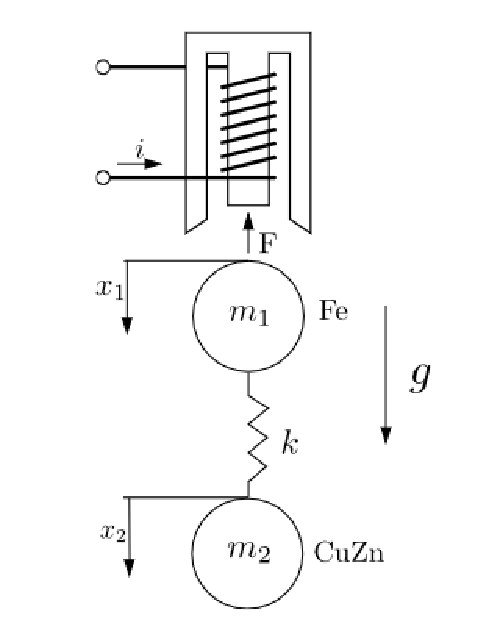
\includegraphics[width=70mm]{two_mass_floating_bodies.pdf}
		\caption{Structure of the Two Mass Floating Bodies Model. \\ \footnotesize{Source: Wang, Xinyu/Erstellung eines Katalogs regelungstechnischer Problemstellungen mit ausführbaren Beispiellösungen }}
	\end{figure}
	
	%variables which are used additional to those in the model equations
	\begin{tabular}{ll}

	\end{tabular}
	
	%%%%%%%%%%%%%%%%%%%%%% MDOEL EQUATIONS %%%%%%%%%%%%%%%%%%%%%%%%%%%
	
	\section{Model Equations} % MUST
	
	State Vector and Input Vector:
	\begin{align*}
		\underline{x} &= (x_1 \ x_2 \ x_3 \ x_4)^T = (s_1 \ s_2 \ v_1 \ v_2)^T \\
		\underline{u} &= u_1 = I
	\end{align*}
	
	\noindent System Equations:			
	\begin{subequations}
	\begin{align}
		\dot{x}_1 &= x_3 \\
		\dot{x}_2 &= x_4 \\
		\dot{x}_3 &= g - \frac{k_f}{m_1}(x_1 - x_2) - k_1\frac{I}{m_1(x_1+k_2)^2}  \\
		\dot{x}_4 &= g + \frac{k_f}{m_2}(x_1 - x_2) \\
	\end{align}
	\end{subequations}

	%%%%%%%%%%%%%%%%%%%%%% PARAMETERS | OUTPUTS %%%%%%%%%%%%%%%%%%%%%%%%%%%
	\noindent
	Parameters: $m_1, \, m_2, \, k_1, \, k_2, \, k_f, \, g$  % variables with constant, predefined value
	\\
	Outputs: $s_2$ % MAY
	
	%%%%%%%%%%%%%%%%%%%%%% ASSUMPTIONS %%%%%%%%%%%%%%%%%%%%%%%%%%%
	
	\subsection{Assumptions} % MAY 
		\begin{enumerate} %possible list type for the Assumptions
			\item Mass of the iron ball is a pointmass.
			\item Mass of the brass ball is a pointmass.
		\end{enumerate}
	
	%%%%%%%%%%%%%%%%%%%%%% EXEMPLARY PARAMETER VALUES %%%%%%%%%%%%%%%%%%%%%%%%%%%	
	
	\subsection{Exemplary parameter values}
	\begin{tabular}{cl}
\hline
  Symbol  & Value                                                                                                                                                                                \\
\hline
   $A$    & $\left[\begin{matrix}0.8189 & 0.0863 & 0.09 & 0.0813\\0.2524 & 1.0033 & 0.0313 & 0.2004\\-0.0545 & 0.0102 & 0.7901 & -0.258\\-0.1918 & -0.1034 & 0.1602 & 0.8604\end{matrix}\right]$ \\
   $B$    & $\left[\begin{matrix}0.0045 & 0.0044\\0.1001 & 0.01\\0.0003 & -0.0136\\-0.0051 & 0.0936\end{matrix}\right]$                                                                          \\
 $B_{1}$  & $\left[\begin{matrix}0.0045 & 0.0044\\0.1001 & 0.01\\0.0003 & -0.0136\\-0.0051 & 0.0936\end{matrix}\right]$                                                                          \\
 $C_{1}$  & $\left[\begin{matrix}1.0 & 0 & -1.0 & 0\\0 & 0 & 0 & 0\\0 & 0 & 0 & 0\end{matrix}\right]$                                                                                            \\
   $C$    & $\left[\begin{matrix}1.0 & 0 & 0 & 0\\0 & 0 & 1.0 & 0\end{matrix}\right]$                                                                                                            \\
 $D_{11}$ & $\left[\begin{matrix}0 & 0 & 0\\0 & 0 & 0\\0 & 0 & 0\end{matrix}\right]$                                                                                                             \\
 $D_{12}$ & $\left[\begin{matrix}0 & 0\\1.0 & 0\\0 & 1.0\end{matrix}\right]$                                                                                                                     \\
 $D_{21}$ & $\left[\begin{matrix}0 & 1.0 & 0\\0 & 0 & 1.0\end{matrix}\right]$                                                                                                                    \\
\hline
\end{tabular}

	%%%%%%%%%%%%%%%%%%%%%% DERIVATION & EXPLANATION %%%%%%%%%%%%%%%%%%%%%%%%%%%	
	
	\section{Derivation and Explanation} % SHOULD
	
	The Lagrangian mechanics was used for the solution.
	
	%%%%%%%%%%%%%%%%%%%%%% REFERENCES %%%%%%%%%%%%%%%%%%%%%%%%%%%
	
	\begin{thebibliography}{10}		
		\bibitem{But21}Wang, Xinyu: 
		\textit{Erstellung eines Katalogs regelungstechnischer Problemstellungen mit ausführbaren Beispiellösungen}, student research project at the Institut of Control Theory TU Dresden, 2021. \\
		(not publicly accessible)
	\end{thebibliography}

\end{document}

